% gm-final-exam.tex

\documentclass[12pt]{article}
% \usepackage{enumerate}
% \usepackage{syllogism} 
\usepackage{october}
% \usepackage[table]{xcolor}
\pagestyle{empty}
\newcounter{frage}
\setcounter{frage}{0}
\newcommand{\frage}[0]{\refstepcounter{frage}\arabic{frage}}

\begin{document}

\textbf{Final Exam}


Show all of your work. Correct answers without showing how to get them
does not earn you points.

\textbf{There are TWO pages and NINE questions.} The maximum number of
points is 100.

({\frage}) Solve the logarithmic equation. Do not use a calculator for your
calculation. It's OK to use a calculator to check your answer. [10]
\begin{equation}
  \label{eq:vuomebic}
  \log_{2}x-\log_{2}\frac{1}{4}=3
\end{equation}

({\frage}) Solve the trigonometric equation in $\{x\in\mathbb{R}|0^{\circ}\leq{}x<360^{\circ}\}$. [12]
\begin{equation}
  \label{eq:waibohng}
  5\cos^{2}x=4\sin{}x+4
\end{equation}

({\frage}) Solve the following system of equations by any method.[10]
\begin{equation}
  \label{eq:tiwiehai}
  \begin{array}{rcccl}
    x&+&\frac{1}{5}y&=&\frac{4}{3} \\
    3x&-&2y&=&-9
  \end{array}
\end{equation}

({\frage}) The points $A$ and $B$ in the figure are on opposite sides
of the river and inaccessible from points $x$ and $y$. Find the
distance $AB$ from the survey notes.

\bigskip

\begin{tabular}{|l|r|}\hline
  distance from $x$ to $y$ & 450ft \\ \hline
  angle at $x$ for triangle $Axy$ & 129$^{\circ}$ \\ \hline
  angle at $y$ for triangle $Ayx$ & 32$^{\circ}$ \\ \hline
  angle at $x$ for triangle $Bxy$ & 43$^{\circ}$ \\ \hline
  angle at $y$ for triangle $Byx$ & 113$^{\circ}$ \\ \hline
\end{tabular}

\begin{figure}[h]
    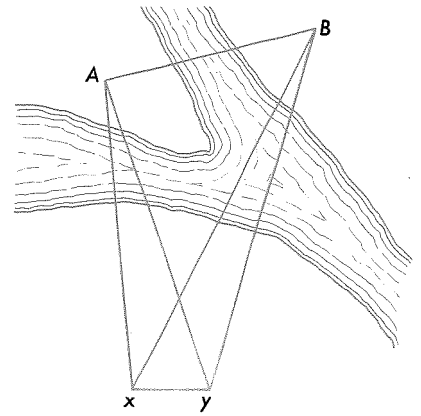
\includegraphics[scale=.5]{./riceknight491a.png}
\end{figure}

\newpage

({\frage}) The time it takes to ride your bicycle from home to work is
normally distributed with a mean of $28.4$ minutes and a standard
deviation of $3.1$ minutes. What is the probability that the bike ride
takes more than half an hour? [10]

({\frage}) Solve the following spherical triangle. Clearly indicate the three
missing items and their solution. Hint: $c$ is greater than
$90^{\circ}$ (use the alternative solution when you take the inverse
sine function of $\sin{}c$). [12]
\begin{equation}
  \label{eq:ooxusahf}
  A=24^{\circ}53'39'',b=32^{\circ}5'34'',C=93^{\circ}40'45''
\end{equation}

({\frage}) Solve the exponential equation. Do not use a calculator for your
calculation. It's OK to use a calculator to check your answer. [10]

\begin{equation}
  \label{eq:vaiphook}
  3^{x-1}=e^{3x}  
\end{equation}

({\frage}) Solve the following right spherical triangle with a right angle at
$A$. [12]
\begin{equation}
  \label{eq:eichaech}
  b=56^{\circ}21'30'',B=59^{\circ}15'32''
\end{equation}

({\frage}) According to 2010 census data, the ratio of men to women among
centenarians is $1:4$ (i.e.\ 20\% of centenarians are men). What is
the probability that out of 50 centenarians 12 or more are male? [12]

\end{document}
